\chapter{Last Speech: Testimony, Scale, and the Work of Arrival}

This lecture is unusual in tone and structure. It is partly a valediction, partly a strategic address, and only gradually does it reveal its mathematical spine. In the curated LazyingArt LLC playlist, reconstructed through Video2Book, the talk survives without validated board images, so the chapter must take its quantitative structure from the transcript itself: bodily recovery, planetary market size, rate mismatch, organizational reach, and the dual logic of training and testimony. We shall therefore let the argument unfold in the order the speaker gives it, moving from ceremony to evidence, from evidence to scale, and from scale to duty.

\section{Prologue: Mark Hughes, Jim Rohn, and Continuity}

The lecture does not begin cleanly with Jim Rohn. It is framed by an emcee who wants us to hear Rohn as something more than an honored guest. He is presented as one of the living continuations of Mark Hughes's original dream, as a figure whose language of integrity, enlarged life, and larger-hearted opportunity remains continuous with the roots of the company.

That prologue matters. It prepares the listener to accept a later shift from applause to calculation. The emcee's own story of family routine, missed Sundays, and the ``church of Jim Rohn'' is not there merely for charm. Its function is to say that Rohn's influence is not cosmetic; it reorganizes a life. Once that framing has been supplied, Rohn can enter the stage not just as a speaker, but as a bearer of institutional memory and moral tone.

Rohn's own opening remains in this warm register. He greets people, thanks them, calls out names and countries, and allows the room to become intimate before it becomes analytical. That is the right order. In a talk built around organizational reach, the audience must first feel itself as a community.

\section{Recovery as Testimonial, Then Scale as Calculation}

Rohn's first serious piece of evidence is not corporate. It is bodily. He tells us that when he first became ill, his weight had fallen to about \(123\) pounds. The regimen is stated very simply:
\begin{align}
W_{\mathrm{start}} &\approx 123\ \text{lb},\\
s_{\mathrm{ill}} &= 3\ \text{shakes/day},\\
\Delta W &> 30\ \text{lb},\\
s_{\mathrm{later}} &= 2\ \text{shakes/day}.
\end{align}
The arithmetic is modest, but the role it plays is large. This is a testimonial before it is a nutrition schedule. The listener is meant to infer that products, people, and prayers have all entered into one concrete recovery.

The lecture then widens from this one body to a much larger question. How many people are contained inside Herbalife's current reach? Rohn asks for a calculation, floats a rough lower bound, corrects upward, and settles on the scale that matters:
\begin{equation}
C = 70, \qquad M > 3\times 10^9,
\end{equation}
where \(C\) is the number of countries and \(M\) the reachable market.

\begin{table}[h]
\centering
\begin{tabular}{p{0.38\linewidth} p{0.34\linewidth}}
recovery starting point & \(W_{\mathrm{start}} \approx 123\ \text{lb}\) \\
recovery regimen & \(3\) shakes/day, later \(2\) \\
weight regained & \(>30\ \text{lb}\) \\
global footprint & \(70\) countries \\
reachable market & \(>3\times 10^9\) people \\
low-income benchmark & \(\$1/\text{day}\) \\
large gathering scale & \(18{,}000\) people
\end{tabular}
\caption{Transcript-backed numerical claims that anchor the lecture's movement from private testimony to global scale.}
\end{table}

\subsection{Question \& Answer}

How does a personal recovery story become a global business argument?

Because the lecture treats testimony as local proof. A change in one life is not the end of the discussion; it is the beginning of a scaling question. If transformation is real here, how many could enter such a transformation elsewhere? The talk moves from one recovered body to 70 countries because it wants to say that the local case is not isolated; it is a model instance.

This is also why the market calculation comes exactly here. It is not pasted in from business school. It is motivated by the testimonial structure itself.

\section{The Market Is Vast, and We Are Still Behind}

The first true paradox of the lecture appears immediately after the large number is stated. One might expect the tone to become congratulatory. Instead Rohn says that no matter how much business is being done, the organization is still behind. That sounds contradictory until he supplies the rate comparison.

His strongest local formulation is memorable because it is so compressed:
\begin{equation}
1\ \text{new customer} \mapsto 3\ \text{new babies}.
\end{equation}
This is not demographic theory in the strict sense. It is a motivational model of lag. The lecture's mathematical point can be written more abstractly as
\begin{equation}
r_{\mathrm{reach}} < r_{\mathrm{need}},
\end{equation}
and therefore the service gap
\begin{equation}
\Delta(t)=N_{\mathrm{market}}(t)-N_{\mathrm{served}}(t)
\end{equation}
need not shrink merely because activity is intense.

\paragraph{Worked example.}
If, over some short interval, the organization reaches one new person while three new units of need appear elsewhere, then
\begin{align}
\Delta N_{\mathrm{served}} &= 1,\\
\Delta N_{\mathrm{new\,need}} &= 3,
\end{align}
so the gap changes by
\begin{equation}
\Delta\Delta=\Delta N_{\mathrm{new\,need}}-\Delta N_{\mathrm{served}}=2>0.
\end{equation}
This is precisely the lecture's intended shock. One may be working hard and still be falling further behind.

\begin{remark}
The inequality \(r_{\mathrm{reach}}<r_{\mathrm{need}}\) and the gap variable \(\Delta(t)\) are editorial reconstructions. They sharpen the speaker's repeated line, ``we're behind,'' but they are not themselves spoken formulas.
\end{remark}

\begin{figure}[h]
\centering
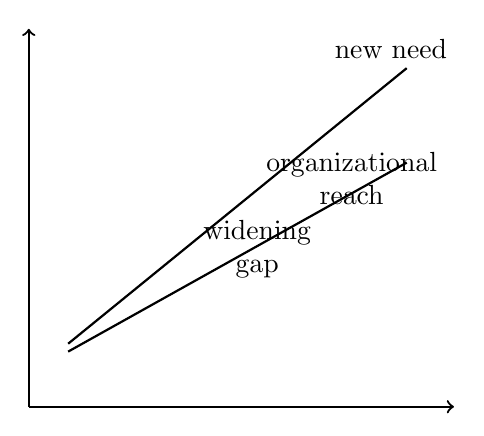
\begin{tikzpicture}[x=1cm,y=1cm]
\draw[->, thick] (0,0) -- (0,4.8);
\draw[->, thick] (0,0) -- (5.4,0);
\draw[thick] (0.5,0.7) -- (4.8,3.1);
\draw[thick] (0.5,0.8) -- (4.8,4.3);
\node[align=center] at (4.6,4.55) {new need};
\node[align=center] at (4.1,2.9) {organizational\\reach};
\node[align=center] at (2.9,2.0) {widening\\gap};
\end{tikzpicture}
\caption{Transcript-only schematic of the lecture's central lag claim: current need grows faster than current reach.}
\end{figure}

\subsection{Question \& Answer}

Why can a rapidly growing organization still honestly say it is behind?

Because growth and adequacy are not the same quantity. The lecture insists on this distinction. A large market, rapid expansion, and real achievement may all be true at once; yet if the arrival of new need outruns the arrival of service, the structural condition remains one of lag. The paradox is not rhetorical excess. It is the quantitative heart of the talk.

\section{Mission as Organizational Arrival}

Once the lag has been established, the lecture refuses to leave it abstract. Rohn translates scale into moral and practical terms by repeating a single pattern: until you get there. Until the organization gets there, people remain overweight, remain caught in health problems, remain economically pinched, remain in despair. In some countries, he says, people are earning only
\begin{equation}
I_{\min}=\$1/\text{day}.
\end{equation}

The key move is that the market is not described as a map of revenue targets. It is described as a waiting population. The function of the organization is therefore arrival. That word is not used as a technical term in the lecture, but the causal logic is unmistakable:
\begin{equation}
\text{organizational arrival} \to \{\text{health},\ \text{income},\ \text{recognition}\}.
\end{equation}
This too is best read cautiously. It is a transcript-guided compression of a repeated spoken sequence, not a theorem of social science.

The same logic underlies the praise of Michael Johnson. Rohn says he does not know how the CEO manages to keep products flowing into 70 countries. The job is called ``impossible.'' Yet this praise is not a digression. It prepares the next step: if the executive job is already at the limit, then distributor responsibility must widen rather than narrow. The burden of reaching the 3 billion is distributed.

\section{Mark's Dream of a Place}

Rohn now shifts from numerical scale to institutional form. What, exactly, did Mark Hughes want to create? Not merely a room. Not merely a hotel. A room is a place in the geometric sense, but not yet in the human sense the lecture is after.

\begin{definition}
In the logic of this talk, a \emph{place} is not first an enclosure but a human field: distributors, stories, welcome, products, memory, and repeated return.
\end{definition}

Rohn's phrasing is cumulative. First it was a family place. Then it became larger than a family. Now it can gather \(18{,}000\) people in one event. The equation that summarizes the corporate expansion is simple:
\begin{equation}
50+20=70,
\end{equation}
with the first \(50\) countries attached to Mark Hughes and the added \(20\) to Michael Johnson. But the more important sentence is conceptual: the place is the people.

\subsection{Question \& Answer}

What is the place that Herbalife is supposed to create?

The lecture's answer is that the place is made out of human participation. It is the distributors, you and me, the persons who hear the story, use the products, improve their health, bless their families, and begin earning money. The hotel hosts the gathering, but it is not the object of the chapter. The human field is.

This is why the lecture can move so naturally from institutional architecture to persuasion. Once the place is understood as a field of persons, the next question is no longer where we meet, but how people are moved within that field.

\section{Training and Testimonials: Head and Heart}

Here the lecture becomes especially crisp. Rohn says that two things matter at this level: training and testimonials. Their functions are distinct, and the distinction is sharp enough to preserve in displayed form:
\begin{align}
\text{training} &\to \text{head},\\
\text{testimonials} &\to \text{heart}.
\end{align}
In editorial shorthand, we may write
\begin{equation}
\text{training} \to \text{understanding}, \qquad
\text{testimonials} \to \text{motivation}.
\end{equation}

This is one of the lecture's clearest local constructions. The training explains, organizes, answers, and informs. The testimonials show that the explanation has already entered somebody's life. Thus the examples of early testimony are always concrete: health has changed, family has changed, money has begun to come in. The transcript-backed map is therefore
\begin{equation}
\text{Herbalife participation} \to \{\text{health},\ \text{family},\ \text{income}\}.
\end{equation}

The historical examples serve the same function. Little London meetings expand into Royal Albert Hall. The scale of the meeting is itself a testimonial. A roomful of people is no longer merely a roomful; it is evidence that the story has already been lived by many.

\begin{table}[h]
\centering
\begin{tabular}{p{0.28\linewidth} p{0.28\linewidth}}
training & testimonials \\
head & heart \\
answers & motivation \\
clarity & proof of change \\
understanding & desire to join and stay
\end{tabular}
\caption{The lecture's two-channel persuasive structure.}
\end{table}

\subsection{Question \& Answer}

Why are both training and testimonials necessary?

Because the lecture does not trust information by itself, nor feeling by itself. One must know what Herbalife is, what it does, and how it works. But one must also see that it has already changed somebody. Training by itself may leave the listener informed but unmoved; testimony by itself may leave the listener moved but ungrounded. The chapter should preserve the pair, not flatten it into a single leadership slogan.

\section{Always Say Yes: The Small-Scale Algorithm of Leadership}

After building upward to billions and outward to 70 countries, the lecture descends to something deceptively small. Suppose a younger person is just beginning leadership training. What should that person do when asked to participate? The answer is repeated until it becomes almost liturgical: always say yes.

The point is not mere obedience. It is that leadership begins below the level of formal teaching. Door duty, handshake, welcome, standing where people come in, speaking briefly, giving a testimonial: these are all elementary acts in which the culture reproduces itself. The lecture's small-scale algorithm can therefore be written as
\begin{equation}
\text{say yes to small tasks} \to \text{hospitality} \to \text{testimonial} \to \text{leadership}.
\end{equation}

\paragraph{Update rule.}
A beginner's passage upward may be rendered as a short rule:
\begin{enumerate}
\item accept the small public task;
\item practice visible hospitality;
\item learn to welcome and steady the room;
\item give a testimonial when asked;
\item become capable, later, of giving training.
\end{enumerate}

This is why the lecture insists that it is not only about learning to give a fine training program. It is also about learning to shake hands, learning to say hello, learning to say welcome. The culture lives first in these minor acts. Only later does it appear as full-scale leadership.

The same section carries the very compressed promise that the fifth day may be the magic day, that next week may be the best week ever, that one should keep doing what one is doing. These phrases are not detachable optimism. They are the local motivational grammar of the culture.

\subsection{Question \& Answer}

What does leadership training look like before one is ready to teach?

It looks like repeated, public, disciplined assent to small responsibilities. The lecture wants us to see that the road to leadership is not hidden behind grand talent. It is built out of yes, yes, yes---to the door, to the greeting, to the handshake, to the room, to the first visible act of care for another person.

\section{Summary}

The chapter begins with ceremony but does not stay there. It moves from institutional memory to bodily testimony, from bodily testimony to market scale, from market scale to a paradox of lag, and from that paradox to organizational duty. The 70 countries and the 3 billion people are not there to decorate the lecture; they define its burden. The world is large enough that success may still leave us behind.

Rohn then answers scale with form and form with method. Mark Hughes's ``place'' is not a building but a human field. Inside that field, training reaches the head, testimonials reach the heart, and leadership begins not at the podium but in the first small yes. The lecture closes as it ought to: not with a solved problem, but with an unfinished mission, still widening outward, still asking for acceleration, reach, and contact.